\documentclass[<options>]{elsarticle}

\usepackage{lineno,hyperref}
\usepackage{longtable,booktabs}
\usepackage{tabu}
\usepackage{listings}
\usepackage[table]{xcolor}



\modulolinenumbers[5]

\journal{Journal of \LaTeX\ Templates}

%%%%%%%%%%%%%%%%%%%%%%%
%% Elsevier bibliography styles
%%%%%%%%%%%%%%%%%%%%%%%
%% To change the style, put a % in front of the second line of the current style and
%% remove the % from the second line of the style you would like to use.
%%%%%%%%%%%%%%%%%%%%%%%

%% Numbered
%\bibliographystyle{model1-num-names}

%% Numbered without titles
%\bibliographystyle{model1a-num-names}

%% Harvard
%\bibliographystyle{model2-names.bst}\biboptions{authoryear}

%% Vancouver numbered
%\usepackage{numcompress}\bibliographystyle{model3-num-names}

%% Vancouver name/year
%\usepackage{numcompress}\bibliographystyle{model4-names}\biboptions{authoryear}

%% APA style
%\bibliographystyle{model5-names}\biboptions{authoryear}

%% AMA style
%\usepackage{numcompress}\bibliographystyle{model6-num-names}

%% `Elsevier LaTeX' style
\bibliographystyle{elsarticle-num}
%%%%%%%%%%%%%%%%%%%%%%%

\begin{document}

\begin{frontmatter}

\title{Towards a standard-based Open Data ecosystem: Analysis of DCAT-AP use at national and European level}

%% or include affiliations in footnotes:
\author[1]{Florian Barth\'el\'emy}
\author[2]{Michael Cochez}
\author[2]{Iraklis Dimitriadis}
\author[2]{Naila Karim}
\author[1]{Nikolaos Loutas}
\author[3]{Vassilios Peristeras}
\author[1]{Brecht Wyns}

\address[1]{PwC Belgium}
\address[2]{Fraunhofer/FIT, Germany}
\address[3]{International Hellenic University, Greece}

\begin{abstract}
In Europe, an open government data ecosystem is being developed. This ecosystem is implemented using various technologies and platforms. The use of a common metadata standard for describing datasets and open data portals, i.e. the DCAT-AP specification, appears as the lingua franca that connects an otherwise fragmented environment. The standard-based consolidation of open data promotes the subsidiarity principle, allowing open data portal owners to choose platforms and internal representations based on their specific requirements as soon as they provide an export with DCAT-AP compliant metadata about the dataset they store. Here, we investigate in depth how the specification is used in practice both at national and at the European level. We identify challenges, opportunities for improvements and issues to be used as input for the next revision cycle of the standard. Our goal is to contribute towards the enrichment of a growing and well-promising European open data ecosystem.
\end{abstract}

\begin{keyword}
open data, metadata, data standards, open data portals, interoperability, DCAT, DCAT-AP
\end{keyword}

\end{frontmatter}

\linenumbers

\section{Introduction and scope}

Governments possess a large amount of basic data which is of critical economic (e.g. (Ahmadi Zeleti et al., n.d.) (Zuiderwijk et al., 2016) and social (e.g. (Ruijer et al., 2017) (Ruijer and Martinius, 2017) value to the society. Along those lines, countries all over the world are developing policies to release this data as Open (Government) Data (Attard et al., 2016) (Zuiderwijk and Janssen, 2014a). In 2003, the European Union (EU) adopted legislation to foster the re-use of Public Data in Member States via the Public Sector Information (PSI) Directive 2003/98/EC (Katleen, 2011), which was revised in 2013 (Directive 2013/37/EU) (Janssen and Hugelier, 2013). The main amendments are the adoption of the "open by default" principle, the breakaway from cost-based charging for PSI towards a marginal cost-oriented fee and increased transparency regarding calculation of the fees, the inclusion of certain cultural institutions as public sector bodies (previously outside the scope), and support for machine-readable and open formats.

In response to the requirements of the revised PSI directive, European public administrations have set up cross-domain and cross-organisational open data portals. These portals have significantly contributed to the establishment of the necessary foundation for a European open data ecosystem, creating value and paving the way towards data-driven governments (Attard et al., 2016), while some of them already support and publish linked data (Ding et al., 2012)  (Ding et al., 2011). Research efforts also exist to “lift” open government portals to the web with the use of web data standards (Waal et al., 2014).

Limitations in real implementations of data portals appeared soon (Attard et al., 2015) (Zuiderwijk and Janssen, 2014b). In addition to the inherent political, cultural, and linguistic diversity in Europe, the development of open data portals has not always been coordinated within and much more across countries. The use of different platforms and the lack of common semantics, metadata (Neumaier et al., 2016) and data models have resulted in a fragmented landscape of open data portals as disconnected information silos, making it hard to exchange metadata between them and interoperate (Janssen et al., 2014). What is more important from the user perspective, citizens and businesses have to query over 150 separate open data portals in Europe if they want to find and combine data and information referring to the whole EU. This situation leads to duplication of information and inconsistencies, it hampers cross-portal search, and limits the discoverability of datasets.

Overcoming the challenges described above, while respecting the subsidiarity principle, was only possible if the different portals with different descriptions of metadata would adhere to a common metadata language. Such a common metadata language, DCAT-AP (DCAT Application Profile), was developed under the Interoperability Solutions for European Public Administrations, Businesses and Citizens (ISA²) Programme of the European Commission, more specifically under its action on promoting semantic interoperability amongst the European Union Member States (SEMIC). By now, it is implemented by the European Data Portal (Carrara et al, 2017), over 15 national data portals and several portals at regional and local level (Klímek et al., 2018).

An Application Profile is a specification that re-uses terms from one or more base standards, adding more specificity by identifying mandatory, recommended and optional elements to be used for a particular application, as well as recommendations for controlled vocabularies to be used. DCAT-AP is mainly based on the Data Catalog Vocabulary (DCAT), which was developed initially at the Digital Enterprise Research Institute in Ireland (Maali et al., 2010) (Cyganiak et al., 2010) and became later a W3C recommendation under the responsibility of the Government Linked Data Working Group\footnote{\href{http://www.w3.org/2011/gld/wiki/Main_Page}{W3C. Government Linked Data (GLD) Working Group.}}. DCAT is an RDF vocabulary designed to facilitate interoperability between data catalogues published on the Web. 

To meet local needs of implementers, it is possible to extend the DCAT Application Profile. The need for such extensions is also mentioned in (Neumaier et al., 2017) where the authors use several web vocabularies to make metadata from open data portals available as linked data. Extensions have already been developed by the EC/ISA\footnote{\href{https://joinup.ec.europa.eu/node/150345/}{Precise guidelines on how to create a valid DCAT-AP extension are available}} Programme for the fields of geospatial (Pellegrino, 2017) and statistical (Dekkers et al., 2016) data: the GeoDCAT-AP spec was developed under the coordination of the Joint Research Center team responsible for the implementation of the INSPIRE Directive, and the StatDCAT-AP spec under the coordination of EUROSTAT. Any DCAT-AP extension should follow strict guidelines. The main aspect of these guidelines is that any data created according to a DCAT-AP extension must also be valid DCAT-AP data. Besides, properties and classes added should not have names which can be easily confused with the ones from DCAT-AP. Finally, properties optional or recommended in DCAT-AP, can be optional, recommended or mandatory in the extension, or be removed completely.

In the current work, we investigate how the DCAT-AP specification is put into practice in Europe. We try to understand better the real-world usage and challenges related to this important initiative to create a European open data ecosystem based on an open standard. We do this both from a standardization as well as a practical usage perspective. Our analysis looks at both national open data portals, with a focus on those which have adapted the DCAT-AP recommendation, and the European Data Portal, which collects data from many national portals. Overall, we found that DCAT-AP is used by already many and an increasing number of portals, that the data collected from portals is reasonably according to the standard, but also that more work is still needed to unify or avoid fragmentation which may be caused by national portals and their extensions. One aspect observed is that often pragmatics win over being interoperable. This is for example the case when portals present their data in various incompatible formats.

The rest of the paper is structured as follows: in chapter 2, we discuss the methodology used for collecting the data. Then we describe our findings for national portals in chapter 3. In chapter 4, we detail our findings for the European Data Portal.  We discuss the findings in chapter 5 and we conclude the paper in chapter 6. Part of this work was published earlier as a technical report.\footnote{\href{https://joinup.ec.europa.eu/document/national-extensions-analysis-dcat-ap}{https://joinup.ec.europa.eu/document/national-extensions-analysis-dcat-ap}}


\section{Methodology}
To analyse the DCAT-AP use and needs in Europe, we studied two aspects. In the first part, we checked the modelling work which has been done by looking into the different national extensions which have been created; the so-called national profiles. Furthermore, we analysed how the corresponding data portals publish their metadata using these profiles. In the second part, we investigated the real use of DCAT-AP properties and classes on the European Data Portal, which collects (i.e., harvests) the metadata from national portals.

\subsection{Analysis of National Extensions}
In the first part of the analysis, we investigate the changes proposed in the formal specification of national profiles. In the second part, we investigate the actual use of these extensions.

For the first part, we manually found and collected the formal specifications from the National DCAT-AP portals shown in Table 1: National DCAT-AP profiles. This had to be done manually as for many portals no directly exportable data formats were available, e.g., a schema file. Moreover, we noticed that even when a formal specification is available as an OWL ontology, there may be still more restrictions in the textual specification. Some of these inconsistencies appear due to limitations in the expressive power of OWL. Some countries maintain a list of updated, added and deleted properties to DCAT-AP. Others have added additional properties or updates to the standard DCAT-AP, but do not explicitly document the changes, making the change identification a rather tedious task. We created an analysis report by comparing each class and property from the national profiles with the usage notes, cardinality, and status (optional, recommended, or mandatory) in DCAT-AP. From this change analysis report we identified updates in properties’ ranges as well as the removal of properties and classes.

Before presenting the overall statistics on the property updates, we present a brief overview of the identified changes per country. We also identify and comment properties updated in many extensions, for example language, licensing, media types, and format. Furthermore, we also inspected whether updates are in accordance with the DCAT-AP extension rules. Non-compliant updates are discussed in part 5.4.

We have included in our analysis the application profiles from the national portal in the table below, chosen by the fact that they have published a DCAT-AP specification. 

\begin{longtabu} to 1.3 \textwidth { | X[l] | }
 \hline
	Belgium - Fedict, OpenKnowledgeBE, \\Web Address:  \url{http://dcat.be/}  \\The information in this analysis is based on communication with Fedict. \\There is no specific information on the website. \\
 \hline
 
	Germany - Finanzbehörde - Geschäfts- und Koordinierungsstelle GovData, \\ Web Address: \url{http://dcat-ap.de/def/}, Version/Update Date: V1.0 2017-06-21 \\ \hline
    
	Ireland-Open Data Unit-Dept of Public Expenditure \& Reform, \\Web Address: \url{https://data.gov.ie/technical-framework}, Version/Update Date: 2015-06-01 \\
\hline

	Italy - AgID - Agenzia per l'Italia Digitale, \\Web Address: \url{https://linee-guida-cataloghi-dati-profilo-dcat-ap-it.readthedocs.io/it/latest/}, \\Version/Update Date: Release 1.0 2017-04-09 Revision 4e3c5e31\\ \hline

	The Netherlands - Kennis- en Exploitatiecentrum Officiële Overheidspublicaties (KOOP), \\Web Address: \url{http://dcat-nl.info/nl/latest/}, \\Version/Update Date: V 1.1 2017-06-01 Revision 120bc7b7\\ \hline

	Norway - Agency for Public Management and eGovernment (Difi), \\Web Address: \url{https://doc.difi.no/dcat-ap-no/}, Version/Update Date: 2016-10-11\\ \hline

	Spain - APORTA INITIATIVE, \\Web Address: \url{http://datos.gob.es/es/documentacion/guia-de-aplicacion-de-la-norma-tecnica-de-interoperabilidad-de-reutilizacion-de}, \\Version/Update Date: 2016-07-28\\ \hline

	Sweden – VINNOVA, \\Web Address: \url{ https://docs.google.com/document/d/17-vEfZXlu9kykcmjXZo1_Z8QKkr7-Prgwd6YUKLRrjk/edit},(restricted access), \\ Version/Update Date: 2016-06-07\\ \hline

	Switzerland - Open Government Data Switzerland, \\Web Address: \url{ https://handbook.opendata.swiss/en/library/ch-dcat-ap},\\ Version/Update Date: 2016-02-09\\ \hline
\\    
\caption{National DCAT-AP profiles}
\end{longtabu}

Next, we analysed the actual use of DCAT-AP in these portals. This proved more difficult than anticipated. Some of these portals do not provide their metadata in any of the standardized RDF serialization formats, but rather in either a platform specific or own customized format. That was an interesting finding. As we focus on interoperability, we decided to only analyse the portals which provide their metadata in a standardized way. That was the case for Ireland, Norway, Spain, Sweden, and Switzerland. 

For these countries, we downloaded the available metadata and measured how often properties on the DCAT-AP Catalog, Dataset, and Distribution are used. To be specific, we measured the fraction of instances which had at least one occurrence of a property. So, when we show the statistic for the \textit{dct:title} property on Dataset, it means that that fraction of the Datasets had at least one value for that property. For DCAT-AP properties which were used by at least one portal on at least 10\% of the instances, we show detailed charts. Other properties are merely listed. Then, for the additional properties used in the respective portals, we also show statistics.

\subsection{Analysis of DCAT-AP use via the European Data Portal}

In order to analyse the real use of DCAT-AP classes and properties in the European data Portal (EDP), SPARQL queries were developed and executed on its SPARQL endpoint i.e. \url{https://www.europeandataportal.eu/sparql}. Given the high number of properties to analyse, the creation of queries was semi-automated using a spreadsheet. The queries were also transformed into URLs and results are automatically loaded, as shown in Fig.1. The queries can be used to monitor the DCAT-AP use or similar models on every portal that has a SPARQL endpoint.

In the example below, we answer to the question ‘how many datasets have a description?’:

\textbf{Class:} dcat:Dataset. \textbf{Property:} dct:description.
\textbf{Query:}
\begin{lstlisting}
PREFIX dcat: <http://www.w3.org/ns/dcat#>
PREFIX dct: <http://purl.org/dc/terms/>
SELECT COUNT(DISTINCT ?s)
WHERE {
?s a dcat:Dataset .
?s dct:description ?o
}
\end{lstlisting}
\textbf{Result: 728196}

\begin{figure}[!h]
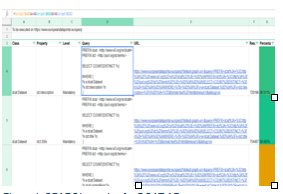
\includegraphics{replace1.png}
\caption{SPARQL queries for DCAT-AP}
\end{figure}

The EDP harvests the metadata from data portals in Europe. These data portals use DCAT-AP in different ways: some are not using DCAT-AP at all, some follow a national DCAT-AP profile and some claim to be fully-compliant with DCAT-AP. The EDP maps these varied uses of DCAT-AP to their own use of DCAT-AP, adding new properties on top of the mappings such as properties under the class dcat:CatalogRecord. These mappings and additions influence the analysis conducted in this part of the study. By querying the EDP endpoint, this analysis assesses only partially the use of DCAT-AP for all data portals harvested by the EDP, as some properties and values from national portals might not be harvested.

The outcomes of this analysis raised a number of questions for the experts of the DCAT-AP working group. These questions were presented and discussed during two webinars on 19/10/2017\footnote{\href{ https://joinup.ec.europa.eu/event/dcat-ap-change-management-release-policy-webinar-19-october-2017-1400-cet}{ https://joinup.ec.europa.eu/event/dcat-ap-change-management-release-policy-webinar-19-october-2017-1400-cet}} and on 08/12/2017\footnote{\href{ https://joinup.ec.europa.eu/event/change-and-release-management-policy-dcat-ap-final-webinar-8-december-2017-1000-cet}{ https://joinup.ec.europa.eu/event/change-and-release-management-policy-dcat-ap-final-webinar-8-december-2017-1000-cet}} .The input received during those webinars is included in the explanations in Chapter 4. In order to further continue the discussion online, topics were created in the DCAT-AP repository on GitHub\footnote{\href{  https://github.com/SEMICeu/DCAT-AP}{  https://github.com/SEMICeu/DCAT-AP}}, where members of the DCAT-AP working group provide their views on the use of different properties and classes and, consequently, on how these elements should be tackled in the next version of DCAT-AP.

Besides the analysis of the use of DCAT-AP classes and properties, a more detailed analysis was conducted for the properties having a controlled vocabulary specified in DCAT-AP. For those properties, a subset of metadata, targeted at large catalogues that use the properties was extracted from the EDP SPARQL endpoint as N-triples. The subset represents 5552 datasets from 6 catalogues harvested by the EDP. For each property supposed to take a value from a controlled vocabulary, two validation checks were done:

\begin{itemize}
\item Confirm the use/non-use of the properties analysed;
\item If the property is used, verify if the value is correctly using the controlled vocabulary or not.
\end{itemize}

For the second check, the DCAT-AP validator\footnote{\href{ http://dcat-ap.semic.eu/dcat-ap_validator.html}{ http://dcat-ap.semic.eu/dcat-ap\_validator.html}} was updated to run validation rules on the metadata. The validation rules analysed automatically if properties start with a specific code list URI, such as \url{http://publications.europa.eu/resource/authority/data-theme/} for the property \textit{dcat:theme} or if the URI contains the correct term category for \textit{dcat:mediaType} from the list maintained by IANA\footnote{\href{  https://www.iana.org/assignments/media-types/media-types.xhtml}{https://www.iana.org/assignments/media-types/media-types.xhtml}}: application/, audio/, font/, example/, image/, message/, text/, video/, etc. 

\section{Analysis of the National Extensions to the DCAT-AP}
DCAT-AP v1.1 covers a basic set of properties and classes for online metadata exchange. To fulfil specific national needs that are not covered by the basic set of properties and classes, DCAT-AP can be extended without losing its compatibility to other DCAT-AP extensions. This extension can include changes, additions or removals in cardinality, classes and properties. Therefore, it is common for extensions to introduce new mandatory properties or move properties from the set of recommended to the set of optional ones. Along with that, extensions can include restrictions by adding cardinality, language and range constraints or even restricting semantics.

\subsection{Analysed DCAT-AP extensions}
The analysis includes the national DCAT-AP extensions for Belgium, Germany, Ireland, Italy, the Netherlands, Norway, Spain, Sweden and Switzerland, as detailed in Table 1. In Fig. 2 the darker colour indicates more changes for the national application profiles. 

\begin{figure}[!h]
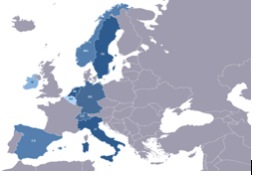
\includegraphics{replace2.png}
\caption{Countries with a national profile based on DCAT-AP. A darker colour indicates more extensive modifications and additions to DCAT-AP.}
\end{figure}

We briefly describe and highlight below significant changes of each extension.

\begin{enumerate}
\item \textit{DCAT-AP.be (Belgium):} DCAT-AP.be does not include any additional properties but allows the data producers to add properties. In addition, each literal has a language tag, apparently to cater for the multilingual requirements in the Belgian context. Used keywords should map to the Data theme Named Authority List of the Publication Office of the European Union\footnote{\href{   http://publications.europa.eu/mdr/authority/data-theme/}{http://publications.europa.eu/mdr/authority/data-theme/}}. Organisations in the metadata get an IRI which derives from the Belgian national company register. The class CatalogRecord is not used in the Belgian extension.

\item \textit{DCAT-AP.de (Germany):} The first version of the German extension of DCAT-AP focuses on copyright, licensing, and law restrictions corresponding to the German context. A 2nd version was announced for 2018.

\item \textit{DCAT-AP (Ireland): }The Irish extension is specified by a data exchange framework, which is based on the DCAT v1.0 profile. The class Dataset is provided with some additional geospatial metadata properties. Some of them have been added to DCAT-AP v.1.1. However, the extension still includes some properties that are not part of DCAT-AP v.1.1

\item \textit{DCAT-AP\_IT (Italy):} The Italian metadata profile DCAT-AP\_IT focuses on granulating the vCard:Kind class to enhance the information metadata for companies. To do so, the class dcatapit:Organization was introduced as a subclass of vCard:Organization, which is in turn is a subclass of vCard:Kind. Additionally to those changes, dcatapit:Organization provides new properties to describe the contact point’s name, email,  telephone number, and URL (e.g., a homepage). Along with the changes to the class vCard:Kind, several other classes were provided with additional properties.

\item \textit{DCAT-AP-NL (the Netherlands): }The Dutch extension of DCAT-AP is called DCAT-AP-NL and was updated in the June 2017. The classes Dataset, Agent, Catalog, Record and Distribution were updated and include some additional properties like registration holder, language and identifier. 

\item \textit{DCAT-AP-NO (Norway):} In the Norwegian DCAT-AP extension, most of the changes took place in the class Dataset and Distribution. The extension provides additional subject, creator, and access right comment properties for the class Dataset. Additionally some properties have been added to describe relations between different datasets. The property dcat:mediaType in the class Distribution was excluded, since it was considered to be the same as dct:format. DCAT-AP-NO also provides a new property dct:identifier for the class Agent.

\item \textit{DCAT-AP-Spain (Spain):} The Spanish DCAT profile was developed and created before DCAT-AP was published and therefore cannot be seen as real extension of DCAT-AP. Given that, the current Spanish standard includes some legacy features, which could cause some interoperability issues with other extensions. In the scope of this analysis we regard the Spanish profile as an extension and describe the different violations against the DCAT-AP v1.1.

\item \textit{DCAT-AP-SE (Sweden):} The DCAT-AP-SE extension of DCAT-AP was developed for öppnadata.se, the Swedish national portal for open data. One focus of the Swedish extension was licensing. Another focus was on restricting the vCard:Kind class to either vCard:Individual or vCard:Organization. In addition, further contact detail properties were added. 

\item \textit{CH-DCAT-AP (Switzerland):} The Swiss extension of DCAT-AP focuses on providing text elements in French, German. Italian and English. It is made mandatory that every text element is provided in each of these languages. 
\end{enumerate}

\subsection{Property changes}
Adding, changing, or removing properties in extensions is common practice. In this overview we group these updates in mandatory, recommended/optional and exclusions of properties. 

\subsubsection{Mandatory changes}
The mandatory property \textit{dct:identifier} was changed most often. Four extensions changed the property for the class Dataset, two for the class Agent and one in the class Standard. For the class Dataset, \textit{dct:identifier} is an optional property. In that case, all four extensions changed it to mandatory.

Like \textit{dct:identifier}, the property \textit{dct:publisher} in class Dataset was changed by four extensions. DCAT-AP v1.1 lists \textit{dct:publisher} as a recommended property, while the extensions changed it to mandatory.

The property \textit{dct:license} was changed by four extensions. Three extensions changed it for the class \textit{Distribution} from recommended to mandatory, while one extension excluded this property and added a new licence attribute with a limited number of possible values. We discuss this property further in part 5.2.

The \textit{dcat:theme} property in class Dataset was changed by four extensions. All of them changed it from an optional to a mandatory property.

The \textit{vcard:fn} property was updated two times for the class Organization and one time for the class Contact. Along with that, \textit{vCard:hasEmail} was changed by three extensions, were two changes took place in the class \textit{Organization }and one in the class \textit{Contact}. Both of these changes restricted the allowed values for vCard properties, where one change was restricting it to organization and the other also allows the use of vCards describing individuals. 

The property \textit{dct:modified} was changed two times in the \textit{Dataset} and \textit{Catalogue} class. For \textit{dct:issued, dcat:mediaType, rdf:type, dct:format, and dcat:accessURL}, two updates were found.
In addition to the changes mentioned above, there is a set of twenty-seven additional changes of mandatory properties. Since all of them were only updated in one profile, we do not discuss them in further detail.

\subsubsection{Recommended and Optional changes}
This section covers the most frequent changed recommended and optional properties. This includes all changes, where a recommended property was changed to an optional and vice versa. The difference between recommended and optional properties is not very strict. Either recommended or optional properties can be left unspecified, with the difference that recommended properties are suggested to be specified to fulfill the EU data interoperability standards. Optional properties however can be left unspecified but could be used to provide additional information about the data and improve the value of it.  

The property \textit{dct:spatial} was changed the most. This includes three changes for the class \textit{Dataset} and one in the class \textit{Catalogue}. Unlike most property changes in section 3.2.1, the changes for \textit{dct:spatial} vary between the different national extensions. Two extensions changed \textit{dct:license} in the class \textit{Dataset} and one change was made in the class \textit{Distribution} and \textit{Catalogue}. The changes of \textit{dct:license} and \textit{dct:spatial} will be discussed in Section 5. 

The property \textit{dct:identifier}  was changed once in the class \textit{Agent} and \textit{Catalogue}. The property \textit{dct:subject }was changed in three extensions. All changes took place in the class \textit{Dataset}. The \textit{vCard:hasTelephone }property was changed two times for the class \textit{Organization} and once for the class \textit{vCard:Contact}. For the class \textit{Dataset}, \textit{dct:creator} was changed two times, while the class \textit{Distribution}  has three and the class \textit{Standard} one change for the property \textit{dct:description}.

Besides the changes mentioned above, there are additionally sixty-three other recommended and optional properties that were changed. Since all the changes took place in only one of the analysed extensions, we will not discuss them any further.

\subsubsection{Exclusion of Recommended and Optional properties}

In some cases, the exclusion of a recommended or optional property is a valid option to improve the national extension of DCAT-AP version. Three of the analysed extensions have excluded such properties, namely DCAT-AP\_IT, DCAT-AP-NL and DCAT-AP-NO.

The Italian extension DCAT-AP\_IT has the most exclusions. For the class \textit{Distribution} the recommended or optional properties \textit{spdx:checksum, foaf:page, dct:language, dct:conformsTo, dct:rights, adms:status,dct:issued} and \textit{dcat:mediaType }are excluded. In the class \textit{Dataset} \textit{dct:relation, dct:source, dct:accessRights, dct:provenance, foaf:page, dct:hasVersion, adms:sample, dct:type,} and \textit{adms:versionNotes} are excluded. Six exclusions were found in the class \textit{Catalogue}, namely \textit{hasPart, isPartOf, dcat:record, dct:spatial, dct:license, and dct:rights} are not included in the extension anymore. In addition \textit{dct:type} is excluded for the class \textit{Agent}.

DCAT-AP-NL and DCAT-AP-NO only excluded properties for the class \textit{Distribution}, where DCAT-AP-NO excluded the \textit{mediaType} and DCAT-AP-NL \textit{license}, \textit{conformsTo, language, page, checksum, type, }and \textit{rights}.

\subsection{Analysis of the use of properties}
In this section, we present the result from measuring the use of properties of the Catalog, Dataset, and Distribution class in the selected national portals. As mentioned, we selected portals with a national profile and where a data dump in a standard RDF format was available. Using these criteria, we ended up with the national portals of Ireland, Norway, Spain, Sweden, and Switzerland. None of these countries use the \textit{CatalogRecord} class. As mentioned, we show charts for properties which were used by at least one portal on at least 10\% of the instances. However, all obligated and recommended properties matching these criteria are included in the charts. We give a short overview of the missing properties, since some of the portals rarely used them.

\subsubsection{Property use in the class Catalog}
The colour code used for the countries is the following:
\begin{figure}[!h]
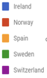
\includegraphics{replace3.png}
\caption{Color code for the countries}
\end{figure}

For the class Catalog all properties were frequently used. However, \textit{dct:hasPart,dct:isPartOf, dcat:record, dct:rights }and\textit{ dct:spatial }were not used at all.
\begin{figure}[!h]
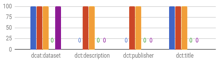
\includegraphics{replace4.png}
\caption{Mandatory properties in the Catalog class}
\end{figure}

\begin{figure}[!h]
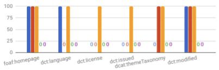
\includegraphics{replace5.png}
\caption{Recommended properties in the Catalog class}
\end{figure}

\begin{figure}[!h]
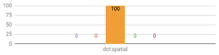
\includegraphics{Replace6.png}
\caption{Optional properties in the Catalog class}
\end{figure}

\subsubsection{Property use in the class Dataset}
The property \textit{dct:conformsTo} occurred rarely in the Spanish and Swiss data dumps. The Swedish data dump was the only one, that used \textit{dct:isVersionOf, dct:provenance, owl:versionInfo} and \textit{adms:versionNotes}. The properties  \textit{dct:hasVersion, adms:sample, dct:type} were not used at all.

\begin{figure}[!h]
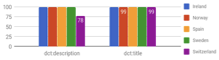
\includegraphics{replace7.png}
\caption{Mandatory properties in the Dataset class}
\end{figure}

\begin{figure}[!h]
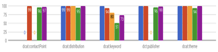
\includegraphics{replace8.png}
\caption{Recommended properties in the Dataset class}
\end{figure}

\begin{figure}[!h]
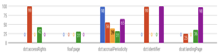
\includegraphics{replace9.png}
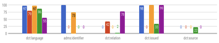
\includegraphics{replace10.png}
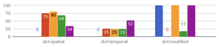
\includegraphics{replace11.png}
\caption{Optional properties in the Dataset class}
\end{figure}

\subsubsection{Property use in the class Distribution}
For the class \textit{Distribution}, \textit{spdx:checksum}, \textit{adms:status} were used by none of the portals. The property \textit{foaf:page} rarely occurred in the Swedish data dump.

\begin{figure}[!h]
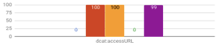
\includegraphics{replace12.png}
\caption{Mandatory properties in the Distribution class}
\end{figure}

\begin{figure}[!h]
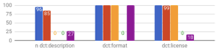
\includegraphics{replace13.png}
\caption{Recommended properties in the Distribution class}
\end{figure}

\begin{figure}[!h]
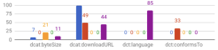
\includegraphics{replace14.png}
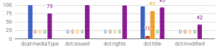
\includegraphics{replace15.png}
\caption{Optional properties in the Distribution class}
\end{figure}

\section{Analysis of DCAT-AP use on the European Data Portal}

\subsection{Analysis of the use of classes and properties}
The collection of data was performed on 10/10/2017 following the methodology described in chapter 2. The results of the queries show that the EDP publishes information about 80 catalogues. These catalogues contain all together 743.746 datasets and 982.771 distributions. Each of the following sub-sections gives an overview of the use of the measured occurrence of properties for the DCAT-AP classes: \textit{dcat:Catalog, dcat:Dataset, dcat:Distribution} and \textit{dcat:CatalogRecord}.

dcat:Catalog

In DCAT-AP, a \textit{catalogue} is defined as a \textit{‘repository that hosts the datasets being described’}. The use of its properties appears in the figures 13-15 below.

\begin{figure}[!h]
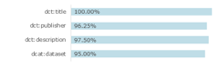
\includegraphics{replace16.png}
\caption{Use of mandatory properties of the class Catalog in the EDP}
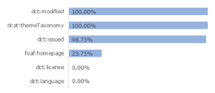
\includegraphics{replace17.png}
\caption{Use of recommended properties of the class Catalog in the EDP}
\end{figure}

\begin{figure}[!h]
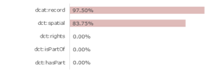
\includegraphics{replace18.png}
\caption{Use of optional properties of the class Catalog in the EDP}
\end{figure}

For the \textit{dcat:Catalog} class, the mandatory properties are respected in almost all cases. Out of the 80 catalogues queried on the EDP:

\begin{itemize}
\item 4 \textit{dcat:Catalog} entries have no dcat:dataset related;
\item 2 \textit{dcat:Catalog} entries have no dct:description attached; 
\item 3 \textit{dcat:Catalog} entries with no dct:publisher attributed, although 2 out of those 3 catalogues have in practice an organisation specified as publisher.
\end{itemize}

The recommended properties, dcat:themeTaxonomy and dct:modified were present in 100\% of the cases, meaning that all the catalogues queried specify at least one theme and a date. The EDP populates these two properties by default:

\begin{itemize}
\item for the theme taxonomy, by using the MDR data themes NAL or a mapping of the data themes harvested to the MDR data themes NAL\footnote{\href{    http://publications.europa.eu/mdr/authority/data-theme/index.html}{ http://publications.europa.eu/mdr/authority/data-theme/index.html}}, as recommended in ‘How to use the MDR data themes vocabulary’\footnote{\href{     https://joinup.ec.europa.eu/release/dcat-ap-how-use-mdr-data-themes-vocabulary}{  https://joinup.ec.europa.eu/release/dcat-ap-how-use-mdr-data-themes-vocabulary }}; and
\item for the modified date, as the latest harvested date of each catalogue by the EDP.
\end{itemize}

Note that this means that even in case national portals do not specify these properties, which happens as we observed in the analysis reported in the previous section, the EDP will present a value.
Almost all the catalogues (98.75\%) also provide the first harvested date with the property dct:issued, and 23.75\% of the catalogues include a homepage. 
An important observation concerning the use of the recommended properties \textit{dct:license} and \textit{dct:language} is that no catalogue specified any of the two properties. The observation on the licence is not in contradiction with the usage note of the property \textit{dct:license} in DCAT for Catalogs. The licence attribute on a catalog refers to the licence of the catalog itself, not of the individual datasets nor distributions.\footnote{\href{      https://www.w3.org/TR/vocab-dcat/\#class-catalog}{https://www.w3.org/TR/vocab-dcat/\#class-catalog}} 

dcat:Dataset
\begin{figure}[!h]
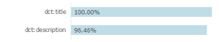
\includegraphics{replace19.png}
\caption{Use of mandatory properties of the class Dataset in the EDP}
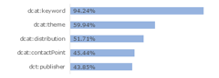
\includegraphics{replace20.png}
\caption{Use of recommended properties of the class Dataset in the EDP}
\end{figure}

The use of mandatory and recommended properties is shown in the figures above. Some interesting findings from the actual use of classes and properties follow.

dct:description not 100\% used

\textit{dct:description} is a mandatory property, yet it is not used on all datasets. This lack of description concerns 3.54\% of the datasets or 26.328 in total. As titles for datasets are often not self-explanatory, data portal owners are encouraged to complete the use of descriptions to improve the understanding and the discoverability of the datasets.

Relationship between Dataset and Distribution

The numbers show that on the EDP, 743.000 datasets have a total of 982.771 distributions. Since a dataset can have several distributions, for example a distribution in CSV format and one in XML, it was expected that the number of distributions would be higher than the number of datasets.
The analysis however shows that not all datasets have a distribution. Only 51.71\% of datasets have distribution(s) defined. This can be explained by the fact that there are other ways to access the data, for example via \textit{dcat:landingPage} (38.42\%) or \textit{foaf:page} (10.31\%), which is often used for geospatial datasets that are accessed through web APIs, such as mapping services.  We also verified that data publishers were not using multiple properties (distribution, landing page and/or page) for the same dataset. The only overlapping use is really minor as it only concerns 17 datasets having at the same time a \textit{dct:landingPage} and a \textit{foaf:page}.

Relationship between dct:publisher and dcat:contactPoint

In the guideline \textit{‘How are publisher and contact point modelled?’}\footnote{\href{ https://joinup.ec.europa.eu/release/how-are-publisher-and-contact-point-modelled }{ https://joinup.ec.europa.eu/release/how-are-publisher-and-contact-point-modelled }} 
, the following recommendation is made:
\textit{‘The way that DCAT and DCAT-AP distinguish between the publisher (the organisation that makes the catalogue or dataset available) and contact information (address where more information can be requested, or feedback can be given) is a continuing source of confusion. It is important to differentiate and provide the two types of information: Publisher is necessary to identify the entity and Contact point allows any person/organisation to communicate and provide feedback.’}

\begin{itemize}
\item As visualised in fig.17, the two properties \textit{dct:publisher} and \textit{dcat:contactPoint} have approximately the same frequency of use (43.85\% and 45.44\%). When analysing more in details if the use of the two properties is aligned with the guideline, we found that among the 38.672 datasets which have both properties defined: 34\% (13.133) have a different publisher than the contact point; and
\item 66\% (25.539) duplicate the information from \textit{dct:publisher} to \textit{dcat:contactPoint}, as specified in the guideline.
\end{itemize}

\begin{figure}[!h]
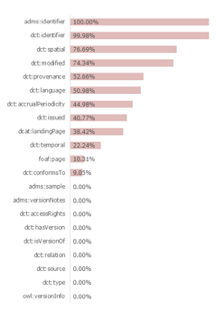
\includegraphics{replace21.png}
\caption{Use of mandatory properties of the class Dataset in the EDP}
\end{figure}

Use of dct:identifier and adms:identifier

DCAT-AP foresees two optional properties for identifying a dataset, \textit{dct:identifier} and \textit{adms:identifier}. While the first one is described as the main unique identifier, e.g. a URI, the second property is provided as a secondary identifier. In practice, the second is used in 100\% of the cases by the EDP itself while the first is in some cases provided by the catalogue of datasets harvested. In most of the cases assessed, the \textit{dct:identifier} follows the same format as the \textit{adms:identifier}. This tends to confirm that the EDP provides a \textit{dct:identifier }and a dataset URI for all the datasets which do not have one already.

Use of dct:spatial
DCAT-AP mandates to use controlled vocabularies for the property \textit{dct:spatial}, independently from the class Dataset or Catalogue, for named places. The list of controlled vocabularies is:

\begin{itemize}
\item MDR Continents Named Authority List\footnote{\href{  http://publications.europa.eu/mdr/authority/continent/}{  http://publications.europa.eu/mdr/authority/continent/}} ;
\item MDR Countries Named Authority List\footnote{\href{  http://publications.europa.eu/mdr/authority/country/}{  http://publications.europa.eu/mdr/authority/country/}} ; and
\item MDR Places Named Authority List\footnote{\href{  http://publications.europa.eu/mdr/authority/place/}{  http://publications.europa.eu/mdr/authority/place/}} .
\item Otherwise, Geonames\footnote{\href{  http://www.geonames.org/}{  http://www.geonames.org/}} URIs.
\end{itemize}

The guideline \textit{‘How should dct:spatial and dct:Location be used?’}\footnote{\href{  https://joinup.ec.europa.eu/release/how-should-dctspatial-and-dctlocation-be-used}{  https://joinup.ec.europa.eu/release/how-should-dctspatial-and-dctlocation-be-used}} reminds also that geographic coordinates can be used to represent a spatial region following the approach described in GeoDCAT-AP. We looked at the use of \textit{dct:spatial}. As shown below, the most used URIs are from Spain (i.e. datos.gob.es) with a local vocabulary, from Flanders (Belgium) with geonames, and from multiple countries with the MDR Countries Named Authority List. The correct use of \textit{dct:spatial} following the controlled vocabularies is detailed in section 4.2. 

\begin{longtable}{*8l}
\rowcolor{blue!90}
\textcolor{white}{\textbf{spatial URI}} & \textcolor{white}{\textbf{Count}} \\ \hline
\rowcolor{gray!10} \url{http://datos.gob.es/recurso/sector-publico/territorio/Autonomia/Pais-Vasco} &4524 \\ \hline
\rowcolor{gray!10} \url{http://sws.geonames.org/3337388} &3824 \\ \hline
\rowcolor{gray!10} \url{http://datos.gob.es/recurso/sector-publico/territorio/Pais/Espa\%C3\%B1a} &3272 \\ \hline
\rowcolor{gray!10} \url{http://sws.geonames.org/3337388/} &3260 \\ \hline
\rowcolor{gray!10} \url{http://datos.gob.es/recurso/sector-publico/territorio/Autonomia/Aragon} &3108 \\ \hline
\rowcolor{gray!10} \url{http://datos.gob.es/recurso/sector-publico/territorio/Provincia/Madrid} &885 \\ \hline
\rowcolor{gray!10} \url{http://datos.gob.es/recurso/sector-publico/territorio/Provincia/Malaga} &837\\ \hline
\rowcolor{gray!10} \url{http://sws.geonames.org/2802361/} &825\\ \hline
\rowcolor{gray!10} \url{https://ruian.linked.opendata.cz/zdroj/st\%C3\%A1ty/1} &653\\ \hline
\rowcolor{gray!10} \url{http://datos.gob.es/recurso/sector-publico/territorio/Autonomia/Galicia} &541\\ \hline
\rowcolor{gray!10} \url{http://datos.gob.es/recurso/sector-publico/territorio/Autonomia/Castilla-Leon } &526\\ \hline
\rowcolor{gray!10} \url{http://sws.geonames.org/2797656/ } &422\\ \hline
\rowcolor{gray!10} \url{http://publications.europa.eu/resource/authority/country/FRA  } &420\\ \hline
\rowcolor{gray!10} \url{http://publications.europa.eu/resource/authority/country/DNK } &415\\ \hline
\rowcolor{gray!10} \url{http://publications.europa.eu/resource/authority/country/EST 	} &414\\ \hline
\rowcolor{gray!10} \url{http://publications.europa.eu/resource/authority/country/SVN } &410\\ \hline
\rowcolor{gray!10} \url{http://publications.europa.eu/resource/authority/country/LVA } &409\\ \hline
\\ 
\caption{Use of dct:spatial for dcat:Dataset}
\end{longtable}

A similar query was run for the class \textit{dcat:Catalog}. The spatial property is used by 33 countries as shown below.

\begin{longtable}{*8l}
\rowcolor{blue!90}
\textcolor{white}{\textbf{spatial}} & \textcolor{white}{\textbf{Count}} & \textcolor{white}{\textbf{spatial}} & \textcolor{white}{\textbf{Count}} & \textcolor{white}{\textbf{spatial}} & \textcolor{white}{\textbf{Count}} \\ \hline
\rowcolor{gray!10} IT &6 &LV &2 &MT &1 \\ \hline
\rowcolor{gray!10} ES &5 &NL &2 &LI &1 \\ \hline
\rowcolor{gray!10} CZ &4 &FI &2 &RS &1 \\ \hline
\rowcolor{gray!10} DE &3 &SI &2 &CY &1 \\ \hline
\rowcolor{gray!10} AT &3 &PT &2 &IE &1 \\ \hline
\rowcolor{gray!10} HR &3 &SE &2 &CH &1 \\ \hline
\rowcolor{gray!10} PL &3 &SK &2 &HU &1 \\ \hline
\rowcolor{gray!10} EE &2 &NO &2 &LT &1 \\ \hline
\rowcolor{gray!10} IS &2 &FR &2 &BG &1 \\ \hline
\rowcolor{gray!10} RO &2 &GB &2 &MD &1 \\ \hline
\rowcolor{gray!10} LU &2 &BE &2 &DK &1 \\ \hline
\\ 
\caption{Use of dct:spatial for the class dcat:Catalog}
\end{longtable}

Use of dct:accrualPeriodicity
We analysed the use of the property \textit{dct:accrualPeriodicity} which indicates the frequency at which a dataset updated by its owner. From the different periodicities with their use, the most used frequencies are visualised below:

\begin{figure}[!h]
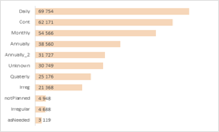
\includegraphics{replace22.png}
\caption{Use of the property dct:accrualPeriodicity}
\end{figure}

Daily, continuously, monthly and annually represent the most used frequency for updating datasets. One important point to notice concerns the quantity of duplicated frequencies, e.g. IRREG and IRREGULAR. For example, some datasets are described using the authority code (i.e. IRREG) provided by the frequency authority list from the Publications Office\footnote{\href{ http://publications.europa.eu/mdr/resource/authority/frequency/html/frequencies-eng.html }{   http://publications.europa.eu/mdr/resource/authority/frequency/html/frequencies-eng.html }} while other datasets use the label from the same authority list (i.e. IRREGULAR). 

52\% of the datasets provide a provenance
The provenance is supposed to be used as for providing a statement about the lineage of a dataset. In a guideline on how to model and express provenance\footnote{\href{  https://joinup.ec.europa.eu/release/dcat-ap-how-model-and-express-provenance}{  https://joinup.ec.europa.eu/release/dcat-ap-how-model-and-express-provenance}}, the following recommendation was made: \textit{‘As the provision of provenance information is not wide-spread and information in free text does not allow further processing, the usefulness of such information in (international) harvesting is questionable and the information may be ignored. Local implementations are of course free to provide provenance information satisfying local requirements.’ }However, the guideline recognises the potential of such information: \textit{‘It could support credibility of a dataset to know which organisation created the metadata for it in the first place and how the description was modified along a chain of exchanges.’}

In practice, the different uses of provenance specified above were observed which demonstrates the fact that the use of this property is not standardised. For example, a dataset\footnote{\href{  https://www.europeandataportal.eu/data/dataset/00dfaddf-f2f0-487a-b28e-aad53a318521}{   https://www.europeandataportal.eu/data/dataset/00dfaddf-f2f0-487a-b28e-aad53a318521}} describes the provenance by mentioning the context and the organisation responsible for the creation of the dataset (translation from Dutch): \textit{‘Label: This map was established on the basis of an inventory during the establishment of the provincial policy for recreational and professional use of waterways.’}
Moreover, the provenance is also used to keep track of the modifications applied to a dataset. One example is \url{https://www.europeandataportal.eu/data/dataset/de-pangaea-dataset864016} with: \textit{‘Label: The data set was checked for completeness, correctness, and consistency of metainformation. Validity of used methods was checked and - if applicable - precision and range of data.’}
Consequently, we would recommend keeping the existing guideline, as it is still relevant.

dcat:Distribution

\begin{figure}[!h]

\includegraphics{replace23.png}
\caption{Use of mandatory properties of the class Distribution in the EDP}
\end{figure}

Relationship between accessURL, downloadURL and Distributions
As the figure above shows, almost all distributions respect the mandatory property \textit{dcat:accessURL}. There was no case for which a distribution had no \textit{accessURL} and no \textit{downloadURL}.

We also looked at the use of the two properties combined, to confirm if this use is differentiated or not. In practice, 16.866 distributions queried have different URLs for access and download while 253.006 distributions\footnote{The number of distributions using downloadURL is slightly different than in the percentage of the visual below (optional property dcat:downloadURL) due of the time gap between queries.}  have the same URL. This shows that the high majority of the distributions using the two properties do not provide different information for both properties but simply copy twice a downloadURL, as explained in the guideline ‘How to use accessURL and downloadURL?’\footnote{\href{   https://joinup.ec.europa.eu/release/how-use-accessurl-and-downloadurl }{   https://joinup.ec.europa.eu/release/how-use-accessurl-and-downloadurl }}.

\begin{figure}[!h]
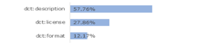
\includegraphics{replace24.png}
\caption{Use of recommended properties of the class Distribution in the EDP}
\end{figure}

Use of licences
Only 27.86\% of the distributions have a licence property defined. This can be a barrier for the reuse of the open data, as many potential users might not take the risk of using distributions without knowing under which conditions they can do it. The EDP also adds that 90\% of the licences of the datasets on the portal are unknown\footnote{\href{    https://www.europeandataportal.eu/mqa-service/en}{ https://www.europeandataportal.eu/mqa-service/en }}. The portal considers a licence as unknown if it is not part of the list of licences provided by CKAN\footnote{\href{     https://www.europeandataportal.eu/en/licence-assistant}{ https://www.europeandataportal.eu/en/licence-assistant }}. Using known licences for the datasets would greatly simplify the work required for potential users before deciding if they can use specific datasets or not.
In general, we also found that the distributions providing a known licence are compliant with the guideline on \textit{‘How to refer to licence documents and licence URIs?’}\footnote{\href{https://joinup.ec.europa.eu/release/dcat-ap-how-refer-licence-documents-and-licence-uris}{  https://joinup.ec.europa.eu/release/dcat-ap-how-refer-licence-documents-and-licence-uris}}. The guideline specifies that licences should always be identified with URIs which should resolve to the description of the licence.

\begin{figure}[!h]
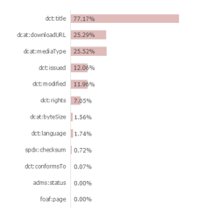
\includegraphics{replace25.png}
\caption{Use of optional properties of the class Distribution in the EDP}
\end{figure}

Relationship between dct:title, dct:format and dcat:mediaType
DCAT-AP recommends to use:

\begin{itemize}
\item \textit{dct:format} to give information about the file format of the distribution;
\item \textit{dcat:mediaType}, as a subproperty of dct:format, to follow the official register of media types managed by IANA\footnote{\href{ https://www.iana.org/assignments/media-types/media-types.xhtml}{   https://www.iana.org/assignments/media-types/media-types.xhtml}}; and
\item \textit{dct:title} to give a name to the distribution.
\end{itemize}

However, our analysis proved that many distributions do the opposite: \textit{dct:title} is in many cases used to inform about the format of the file instead of \textit{dct:format}. 

Despite this misuse, when looking at the combined use of \textit{dct:title} and \textit{dcat:mediaType}, most of the distributions observed use appropriately the two properties: \textit{dct:title} as a name for the distribution and \textit{dcat:mediaType} with a value from IANA.

Some members of the DCAT-AP community have expressed a preference to use only \textit{dct:format} with IANA media type. One reason for using IANA media types, is that you can express the \textit{innerMimeType} for Zip-Files. On the other hand, \textit{dct:format} is more flexible. Even though IANA does not include all geospatial values, they can be added to the OP list (\textit{dct:format}). Chapter 4.2 goes deeper in the analysis of the controlled vocabularies for \textit{dct:format} and \textit{dcat:mediaType}. 

dcat:CatalogRecord
DCAT-AP defines the class Catalog Record as \textit{‘a description of a dataset’s entry in the catalogue’}. The analysis shows a 100\% use of mandatory properties and recommended properties\textit{ dct:issued }and \textit{adms:status}. Other properties are not used at Catalogue Record level.

\subsection{Analysis of controlled vocabulary use on the European Data Portal}
In DCAT-AP version 1.1, 15 properties are expected to use controlled vocabularies as summarised below: 

\begin{longtable}{*8l}
\rowcolor{blue!90}
\textcolor{white}{\textbf{Property}} & \textcolor{white}{\textbf{Class}} & \textcolor{white}{\textbf{Used on the EDP?}} & \textcolor{white}{\textbf{Controlled Vocabulary}} \\ \hline
\rowcolor{gray!10} dct:language (section 4.1) &Dataset &Yes &MDR Languages Named Authority List \\ \hline
\rowcolor{gray!10} dcat:accrualPeriodicity (section 4.2) &Dataset &Yes &MDR Frequency Named Authority List \\ \hline
\rowcolor{gray!10} dct:theme (section 4.3) &Dataset &Yes &Dataset Theme Vocabulary \\ \hline
\rowcolor{gray!10} dct:publisher (section 4.4) &Dataset &Yes &MDR Corporate bodies Named Authority List \\ \hline
\rowcolor{gray!10} dct:publisher (section 4.4) &Catalog &Yes &MDR Corporate bodies Named Authority List \\ \hline
\rowcolor{gray!10} dct:format (section 4.5.1) &Distribution &Yes &MDR File Type Named Authority List\\ \hline
\rowcolor{gray!10} dcat:mediaType (section 4.5.2) &Distribution &Yes &IANA Media Types \\ \hline
\rowcolor{gray!10} dct:spatial (section 4.5.3) &Dataset &Yes &MDR Continents Named Authority List, MDR Countries Named Authority List, MDR Places Named Authority List, Geonames \\ \hline
\rowcolor{gray!10} dct:spatial (section 4.5.3) &Catalog &Yes &MDR Continents Named Authority Lis , MDR Countries Named Authority List, MDR Places Named Authority List, Geonames \\ \hline
\rowcolor{gray!10} adms:status (section 4.5.4) &CatalogRecord &Yes &ADMS change type vocabulary \\ \hline
\rowcolor{gray!10} dcat:themeTaxonomy (section 4.5.5) &Catalog &Yes &Dataset Theme Vocabulary \\ \hline
\rowcolor{gray!10} dct:language &Catalog &No &MDR Languages Named Authority List \\ \hline
\rowcolor{gray!10} adms:status &Distribution &No &ADMS status vocabulary \\ \hline
\rowcolor{gray!10} dct:type &Agent &No &ADMS publisher type vocabulary \\ \hline
\rowcolor{gray!10} dct:type &LicenseDocument &No &ADMS licence type vocabulary \\ \hline

\\ 
\caption{Comparison between the list of properties supposedly using Controlled Vocabularies and the lists of properties present on the EDP}
\end{longtable}

The 4 properties not used on the EDP are not analysed in this chapter but have dedicated descriptions in chapter 4.1:

\begin{itemize}
\item adms:status for the class dcat:Distribution. This is not an issue as the property is optional.
\item dct:type for the class foaf:Agent. This mandatory class defines the range of the properties publisher (dct:publisher) on Dataset and Catalogue. It has two properties, foaf:name and dct:type. dct:type is recommended and is used to refer to a type of the agent that makes the Catalogue or Dataset available. The class agent is extensively used even though the type property is not provided for this class.
\item dct:type for the class dct:LicenseDocument. The recommended class License Document defines the range of the property dct:license on classes Catalogue and Distribution. As the class is not used by the EDP, the property dct:type for indicating the type of licence is not used either.
\item dct:language for the class dcat:Catalog. This recommended property is not used for the class Catalog on the EDP as shown in section 3.3.1.
\end{itemize}

In Table 4, the first 11 properties present on the EDP, marked with “Yes” were analysed. Automated analyses were conducted for 9 out of the 11 properties with the help of the DCAT-AP validator\footnote{\href{  http://dcat-ap.semic.eu/dcat-ap\_validator.html }{    http://dcat-ap.semic.eu/dcat-ap\_validator.html}}. The 2 remaining properties, dct:publisher for the class dcat:Dataset and the same property for the class dcat:Catalog, were analysed manually. 
The table below summarises the findings for the different properties supposedly using controlled vocabularies. The results are based on a sample of 5.552 datasets from 6 catalogues. An error is recorded when an instance that is supposed to refer to a controlled vocabulary, is not referring or is wrongly referring to a controlled vocabulary.

\begin{longtable}{*8l}
\rowcolor{gray!10}{\textbf{Property}} & {} & {\textbf{Instances in sample}} & {\textbf{Errors}} \\ \hline
\rowcolor{gray!10}{Distribution} & {} & {} & {} \\ \hline
\rowcolor{orange!20} dct:format &Recommended &1859 &\textbf{1859} \\ \hline
\rowcolor{orange!20} dcat:mediaType &Optional &1365 &\textbf{55} \\ \hline
\rowcolor{white!10} adms:status &Optional &0 &\textbf{0} \\ \hline
\rowcolor{gray!10}{Dataset} & {} & {} & {} \\ \hline
\rowcolor{white!10} dct:publisher &Recommended &0 &\textbf{0} \\ \hline
\rowcolor{white!10} dcat:theme &Recommended &5009 &\textbf{0} \\ \hline
\rowcolor{white!10} dct:accrualPeriodicity &Optional &992 &\textbf{0} \\ \hline
\rowcolor{white!10} dct:language &Optional &445 &\textbf{0} \\ \hline
\rowcolor{orange!20} dct:spatial &Optional &3002 &\textbf{3002} \\ \hline
\rowcolor{gray!10}{Agent} & {} & {} & {} \\ \hline
\rowcolor{white!10} dct:type &Recommended &0 &\textbf{0} \\ \hline
\rowcolor{gray!10}{CatalogRecord} & {} & {} & {} \\ \hline
\rowcolor{orange!20} adms:status &Recommended &5536 &\textbf{5536} \\ \hline
\rowcolor{gray!10}{LicenseDocument} & {} & {} & {} \\ \hline
\rowcolor{white!10} dct:type &Recommended &0 &\textbf{0} \\ \hline
\rowcolor{gray!10}{Catalog} & {} & {} & {} \\ \hline
\rowcolor{white!10} dct:publisher &Mandatory &0 &\textbf{0} \\ \hline
\rowcolor{white!10} dct:language &Recommended &0 &\textbf{0} \\ \hline
\rowcolor{orange!20} dct:themeTaxonomy &Recommended &6 &\textbf{6} \\ \hline
\rowcolor{orange!20} dct:spatial &Optional &6 &\textbf{6} \\ \hline
\\
\caption{Number of errors found per property using controlled vocabularies }
\end{longtable}

dct:language on dcat:Dataset

The property \textit{dct:language} for the class \textit{dcat:Dataset} is used to indicate a language for a dataset. DCAT-AP requests implementers to provide a value from the MDR Languages Named Authority List\footnote{\href{   http://publications.europa.eu/mdr/authority/language/}{    http://publications.europa.eu/mdr/authority/language/}} such as \\
\textit{$<$http://publications.europa.eu/resource/ authority/language/ENG$>$} for English. In our sample, only one catalogue uses \textit{dct:language} for the class Dataset pointing correctly to the MDR Languages Named Authority List. The other catalogues are not specifying the language for the class \textit{dcat:Dataset}.

dct:accrualPeriodicity on dcat:Dataset

Similarly, the property \textit{dct:accrualPeriodicity} is used to refer to the frequency at which the Dataset is updated. DCAT-AP requests to use the MDR Frequency Named Authority List\footnote{\href{    http://publications.europa.eu/mdr/authority/frequency}{     http://publications.europa.eu/mdr/authority/frequency}} , for example with a URI value as follows: \textit{$<$http://publications.europa.eu/resource/authority/frequency/ANNUAL$>$}. Among the 6 catalogues analysed, a single one provided information about the frequency of update, providing the correct value from the MDR Frequency Named Authority List.

dcat:theme on dcat:Dataset
The property \textit{dcat:theme }refers to a category of the Dataset. A Dataset may be associated with multiple themes. As for the previous properties, a Controlled Vocabulary must be followed, the MDR data theme Named Authority List\footnote{\href{     http://publications.europa.eu/mdr/resource/authority/data-theme/html/data-theme-eng.html}{      http://publications.europa.eu/mdr/resource/authority/data-theme/html/data-theme-eng.html}}  with a URI pointing to one authority code from the list. From our sample analysis, the Controlled Vocabulary is perfectly used by all 6 catalogues.

dct:publisher on dcat:Dataset and dcat:Catalog

The property \textit{dct:publisher} must follow the MDR Corporate bodies Named Authority List\footnote{\href{      http://publications.europa.eu/mdr/authority/corporate-body/}{       http://publications.europa.eu/mdr/authority/corporate-body/}} for which DCAT-AP specifies that it \textit{“must be used for European institutions and a small set of international organisations. In case of other types of organisations, national, regional or local vocabularies should be used”}\footnote{\href{       https://joinup.ec.europa.eu/release/dcat-ap-v11}{    https://joinup.ec.europa.eu/release/dcat-ap-v11 }}. As data portals can indicate national or subnational publishers, this property could not be verified automatically with the DCAT-AP validator. However, from manual processing, the following conclusions were found:

\begin{itemize}
\item 5 of 6 catalogues give information about \textit{dct:publisher} for the class Dataset;
\item None of the 5 catalogues is using the MDR Corporate bodies Named Authority List. Instead, for 4 catalogues, a URI pointing to the properties \textit{foaf:name}, and \textit{rdf:type} is given. For the URIs of one of those 4 catalogues, the property \textit{foaf:mbox} (i.e. mailbox) is also provided. The fifth catalogue gives the URI of a separate code list maintained independently from the MDR Corporate bodies.
\item For the class \textit{dcat:Catalog}, all catalogues analysed also provide information about \textit{dct:publisher} using a URI pointing to \textit{foaf:name} and \textit{rdf:type}, therefore not using a Controlled Vocabulary as specified by DCAT-AP.
\end{itemize}

Wrongly used properties
The following properties were wrongly used by all catalogues in our sample, as explained in the following sections: 
\begin{itemize}
\item \textit{dct:format} for \textit{dcat:Distribution};
\item \textit{dcat:mediaType} for the class \textit{dcat:Distribution}; 
\item \textit{dct:spatial} for \textit{dcat:Dataset} and \textit{dcat:Catalog}; 
\item \textit{adms:status} for \textit{dcat:CatalogRecord}; and 
\item dcat:themeTaxonomy for dcat:Catalog.
\end{itemize}

dct:format on dcat:Distribution

The \textit{dct:format} property must refer to the MDR File Type Named Authority List\footnote{\href{    http://publications.europa.eu/mdr/authority/file-type/}{        http://publications.europa.eu/mdr/authority/file-type/}} for describing the file format of a distribution. All 6 catalogues have datasets with the property \textit{dct:format}. For all instances identified using \textit{dct:format}, the MDR controlled vocabulary is not followed. Instead, the 
value gives a URI pointing to an instance of \textit{dct:MediaTypeOrExtent} with the format described as a literal in \textit{rdf:label}, e.g. \textit{“WMS”}.

dcat:mediaType on dcat:Distribution
\textit{dcat:mediaType }is a subproperty of \textit{dct:format} used to express the media type of the Distribution as defined in the official register of media types managed by IANA\footnote{\href{     http://www.iana.org/assignments/media-types/media-types.xhtml}{         http://www.iana.org/assignments/media-types/media-types.xhtml}}. Only one catalogue out of 6 uses \textit{dcat:mediaType}. The values provided for the subproperty are almost always correct, with a percentage error of 4\% (55/1365). For the errors identified, a media type not referenced in IANA was used, such as ‘xml/soap’.

dct:spatial on dcat:Dataset and dcat:Catalog
For \textit{dct:spatial} under the class \textit{dcat:Dataset}, multiple Controlled Vocabularies are requested by DCAT-AP, respectively:
\begin{itemize}
\item MDR Continents Named Authority List\footnote{\href{http://publications.europa.eu/mdr/authority/continent/
}{Publications Office of the European Union. Metadata Registry. Authorities. Continents.}} for continents;
\item MDR Countries Named Authority List\footnote{\href{http://publications.europa.eu/mdr/authority/country/}{Publications Office of the European Union. Metadata Registry. Authorities. Countries.}} for countries;
\item MDR Places Named Authority List\footnote{\href{    http://publications.europa.eu/mdr/authority/place/}{Publications Office of the European Union. Metadata Registry. Authorities. Places.}} for places; and
\item Geonames URIs if a particular location is not in one of the mentioned Named Authority Lists.
\end{itemize}

Among the 4 catalogues expressing \textit{dct:spatial}, two types of inconsistencies were identified:
\begin{itemize}
\item 1.719 instances out of 3.002 contain a URI pointing to \textit{locn:geometry} with coordinates and to \textit{rdfs:type} with \textit{dct:Location}; and
\item For 1.283 instances out of 3.002, \textit{dct:spatial} points to a list of territories specific to the country of the catalogue and not following the Controlled Vocabularies provided by DCAT-AP.
\end{itemize}

The same use is expected from the catalogues for the class \textit{dcat:Catalog}. In the sample, the 6 instances analysed use an acronym (e.g. “XY”) of the country of the catalogue instead of pointing to the MDR Countries Named Authority List or another Controlled Vocabulary listed by DCAT-AP.

adms:status on dcat:CatalogRecord
The property \textit{adms:status }for the class \textit{dcat:CatalogRecord} refers tothe type of the latest revision of a Dataset's entry in the Catalogue. All the catalogues analysed use it and all the instances of this property, or 5.536, have the value \textit{“:modified”} in place of one from the list provided by DCAT-AP: \textit{:created, :updated, :deleted}. The ratio and the similar value among all the catalogues selected seem to demonstrate the use of this property by the EDP itself and not by the catalogue owners.

dcat:themeTaxonomy on dcat:Catalog
The property \textit{dcat:themeTaxonomy} for the class \textit{dcat:Catalog} follows the same Controlled Vocabulary than \textit{dcat:theme} for the class Dataset. All catalogues in the sample do not appropriately use the property. All of them indicate the correct first part of the URI, \\
\textit{$<$http://publications.europa.eu/resource/authority/data-theme$>$}, but not the full URI expected with the authoritative code, such as \\ \textit{$<$http://publications.europa.eu/resource/ authority/data-theme/\textbf{AGRI}$>$}. As described in section 3.1, \textit{dcat:themeTaxonomy} is populated by the EDP for all catalogues harvested.

\section{Discussion}
We organise the discussion part based on the major findings we had from our analysis. More specifically we discuss the language support, the licensing metadata, the identified non-conformant changes, coverage for geospatial properties, and the relationship properties between Catalogues, Datasets, and Distributions.

\subsection{Language}
Some national extensions provide multi language support. In particular, Switzerland extension has added xml:lang attribute, to support multilingual elements. The example shown in Figure 2 shows the use aforementioned attribute. This example is taken from Switzerland National DCAT-AP website.

\begin{figure}[!h]
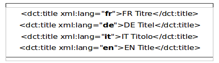
\includegraphics{replace26.png}
\end{figure}

The Spanish DCAT-AP is using dc:language instead of  dct:language. The range of the language attribute is rdfs:Literal, unlike dct:LingusiticSystem in DCAT-AP. Spanish data profile is older than DCAT-AP, and it might be the reason of this inconsistency.  

\subsection{Licence}
Licence and copyrights information has been updated in many national application profiles. German extension has suggested the addition of attribution text for licence, till then it will use dcatde:licenseAttributionByText. The attribute dct:license for class Distribution has been made mandatory in German, Italian, and Swiss application profiles. The Dutch extension consider it unnecessary for class Distribution, therefore they removed it from this class. But added it to the class Dataset, but a small set of possible values. The reason behind this change is the fact, multiple distribution of the same Dataset share same licence. A Distribution with a different licence, will be handled as a different Dataset by Dutch application profile as mentioned in issue report Joinup1. Although in this way Dutch profile can support distributions with different licences, but this approach is not consistent with other national application profile. Therefore, any other national catalogue harvesting data from Dutch profiles needs special work around to capture this information. 
A recommended licence property associated with Catalogue, describe the reuse of the Catalogue itself.  This property is made mandatory in Spanish extension. Making catalogue a mandatory property makes the reuse of the Catalogue clearer, but this update is limited only to Spanish application profile. Although this change, will not incur huge overhead, as the number of Catalogue compared to the Dataset and Distribution are very small.

\subsection{dcat:mediaType and dct:format}
dcat:mediatype is defined as an optional sub property of the recommended property dct:format for class Distribution both in DCAT and DCAT-AP1.1. This property helps in choosing the type of software that could be used to process data. Norwegian application profile has excluded dcat:mediaType with the consideration dct:format is enough to capture the type of Dataset’s Distribution. Similarly Swedish DCAT-AP extension has discouraged the use of dcat:mediaType, as dct:format is enough to capture this information, while the Swiss application profile has made it a recommended property of Distribution. Concluding, we believe the changes made by local implementers regarding the use of dcat:mediaType and dct:format are contradictory. Looking at the different types update made to mediaType property, it seems more appropriate to keep dcat:mediaType optional, as defined in DCAT-AP v1.1.”

\subsection{Non-conformant Changes}
DCAT-AP has defined a clear set of rules for extension. According to the extension rules updates that generalize an existing property or a class might cause inconsistencies and therefore should be avoided. Similarly changing a mandatory property to an optional one, by relaxing cardinality constraints might result in data integration problem, therefore should be avoided. Any update that is not in alliance with extension rule is identified as a non-conformant update in this analysis. Three cases of such updates are presented below:

\begin{itemize}
\item DCAT-AP-NL: The application profile has added a new property version, while there is already a property with same name, but a different property URI. Introducing similar properties and classes is discouraged in DCAT-AP extension rules.
\item CH-DCAT-AP: This national profile has introduced an attribute dcat:coverage, similar to the existing spatial property dct:coverage in DCAT. It seems more like an error rather an update, but the fact that makes it more dubious is the suggestion to avoid the usage of this property.   
\item DCAT-AP-Spain: The national application profile of Spain is older than DCAT-AP1.1, therefore there are some inconsistencies among the two. In particular the difference in adding support for multiple language might cause interoperability issues with other application profiles. 
\end{itemize}

\subsection{Geospatial Properties}
Additional geospatial metadata elements are found in few of the national extensions. In Irish AP, there are three additional spatial attributes associated with the class Dataset. These additional attributes are \textit{GeographicBoundingBox}, \textit{SpatialReference System}, and \textit{Spatial Resolution}. Similarly \textit{politicalGeocodingLevelURI}, \textit{politicalGeocodingURI}, and \textit{geocodingText }are added to German profile. Geometry and \textit{geographicalIdentifier}, \textit{geographicalName }are added the Italian application profile. It has further added some restrictions on the loc:geometry attribute, by associating \textit{CRS}, \textit{Coordinates} and geometry type  as mandatory properties.

The property dct:spatial in DCAT-AP1.1 is used to define geographic coordinates system of a Catalogue.Norway, Spain, Sweden, Switzerland and Netherlands has introduced spatial as an attribute for class Dataset. Sweden has also made it more restricted for class Catalogue. There are many updates in national extension for this property, which makes it a suitable candidate for the new versions of DCAT and DCAT-AP1.1.

\subsection{Relationships between Catalogues, Datasets, and Distributions}
DCAT-AP1.1 has few relationship attributes for class\textit{ Catalogue} and \textit{Dataset}. Relationship properties are used to represent association between catalogues. It could be used to represent inheritance or containment among different \textit{Catalogue} instances. A \textit{Catalogue} is a physical or logical part of another \textit{Catalogue} could be showed using \textit{dct:isPartOf}. A Catalogue contains another Catalogue as a physical or logical part could be represented using the inverse property \textit{dct:hasPart}. Similarly \textit{dct:isVersionOf }is used to describe adaptation, version of or edition association among two datasets. More properties could be added to show different possible association among\textit{ Dataset}, \textit{Catalogue} and \textit{Distribution}. The analysis shows, relationship properties are mostly added in the application profiles of Norway and Spain.

These properties could also play a very important role in data integration and data interoperability, therefore this section also includes other pathways that could be of interest for data publishers, along with listing the observation made in the analysis. One possible use case might be publishing an updated version x of an existing resource y, while maintaining backward compatibility. The use of Relationship properties in such case might help to indicate the fact that x is an updated version of particular resource y and resource y could show the inverse relation by stating y is an older version of x. It should be noted that \textit{dct:versionOf} could be used in this case, but the semantics are too broad. It is also observed that \textit{replace} and \textit{isReplacedBy} properties are only included in the application profile of Norway. This pair of properties is particularly useful to show, if a dataset has become obsolete and another dataset could be used as a replacement.

Another possible prospect of using relationship among DCAT classes is back tracking a \textit{Distribution}, to a \textit{Dataset} and then in turn to a \textit{Catalogue}. In existing application profiles tracking this type of linkage is not easy, as there are not enough attributes to support it. A dataset as standalone entity is not much useful, unless it is possible to investigate its relationship with other datasets. Hence a way to show this association explicitly using properties like \textit{isPartOf/hasPart }would be very helpful. Similarly in some cases a \textit{Dataset} could only be interpreted correctly, with the help of another \textit{Dataset}, requires and \textit{isRequiredBy} are added in Norwegian profile to represent this type association. Another similar type of relation is references and isRefrencedBy added in Norwegian extension. It could be used by a \textit{Dataset} to show reference to another \textit{Dataset} and vice versa. Spain has also added a property named reference to support it.


\section{Future work and conclusion}
In this report, the analysis of national profiles implementing DCAT-AP v1.1 has been presented together with the actual use of the specification both from several national open data portals and the European Data Portal. 

Through our analysis, we have indicated several properties which could be discussed for inclusion in the next iteration of DCAT-AP or the W3C DCAT recommendation. New properties to be considered for future revisions of DCAT-AP include those related to spatial properties and relationships between the class \textit{Dataset} and \textit{Distribution}.

We also found examples of already existing properties which have been modified frequently including, \textit{dct:identifier}, \textit{dct:publisher}, \textit{dcat:theme}, and the way to use the \textit{vCard }class. Moreover, we identified a need to standardise how \textit{license} and \textit{mediaTypes} \textit{formats }are used. 

We also found several changes made by national profiles which limit interoperability or which only help implementations capable of dealing with these specific requirements, while other implementations ignore the information as they are unable to interpret it. 

In the future, the ISA² Programme could help DCAT-AP implementers overcome these interoperability challenges by, for example, creating additional guidelines that ensure the compatibility of extensions with DCAT-AP and the interoperability of extensions among each other, or by checking the compliance of national extensions with DCAT-AP.

An interesting direction for relevant research could include the investigation of the actual use of the vocabularies and other data standards inside the different platforms, to identify best practices around standards usage. 

Moreover, analysis and comparison of data dumps extracted from European Data Portal to that of National DCAT-AP profile could demonstrate the Δ between what exists at the national level and what becomes available at the European one. 

Establishing a standard format for the representation of national DCAT-AP profiles could the identification and documentation of changes easier. Some countries publish for this purpose a pdf file, while others in an html web page. Some of them explicitly document the updates and additions, while others maintain one huge list of properties. For us, it was a tedious job to identify changes.
 
Last, a possible association would be to show succession. An example would be the yearly water consumption report of a country. Representing it using \textit{dct:isVersionOf }deludes the real semantics. Because a new yearly report is just sequence of the dataset. It is not really a version of the last year’s report, nor does it replace the previous one. This type of temporal sequencing doesn’t exist in DCAT-AP1.1, and we didn’t find it in any of the national extensions. 

\section{Acknowledgements}
We would like to thank Makx Dekkers for reviewing the part where the European Data Portal analysis is presented.



\section{Bibliography}
\cite{ahmadi,Attard:2016:DDG:3081418.3081424,ATTARD2015399,Cyganiak:2010:SLG:1839707.1839754,DekkersEtAl:SemStats2016,Ding2011TWCLA,Ding:2012:LOG:2360752.2360982,EJLT238,Janssen:2014:IBO:2780225.2780310,pub.1052835103,KLIMEK20181,maali:hal-01056576,neum-etal-LDOW2017,Neumaier:2016:AQA:3012403.2964909,pellegrino2017,RUIJER201745,ruijer,DBLP:series/lncs/WaalWEJMW14,carrara,ZUIDERWIJK201417,Zuiderwijk2014TheNE,DBLP:journals/polity/ZuiderwijkJKP16}.

\bibliography{mybibfile}

test esto es una prueba
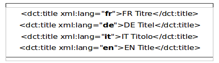
\includegraphics[]{replace999.png}

\end{document}